\documentclass[a4paper]{article}

%% Language and font encodings
\usepackage[english]{babel}
\usepackage[utf8x]{inputenc}
\usepackage[T1]{fontenc}

%% Sets page size and margins
\usepackage[a4paper,top=3cm,bottom=2cm,left=3cm,right=3cm,marginparwidth=1.75cm]{geometry}

%% Useful packages
\usepackage{amsmath}
\usepackage{graphicx}
\usepackage[colorinlistoftodos]{todonotes}
\usepackage[colorlinks=true, allcolors=blue]{hyperref}
\usepackage{tikz}
\usepackage{verbatim}

% we want ER + above/below + left/right
\usetikzlibrary{er,positioning}


\title{DBS Projektdocumentation}
\author{}

\begin{document}
\maketitle

%Brauchen wir ein Abstract?
%\begin{abstract}
%Your abstract.
%\end{abstract}

\section{Projectdokumentation}

Ziel des Projects ist die Entwiklung einer Webanwendung, um einige Daten über die Tweets der Kadidaten der US-Amerikanischen Wahlen auszuwerten. \\
Die Mitarbeiter an diesem Projekt sind:
\begin{itemize}
\item [...]
\end{itemize}
Der ganze Quellcode ist auf \href{https://github.com/0rC0/DBS-election}{https://github.com/0rC0/DBS-election} zu finden. 

\section{Explorative Datenanalyse}

Der Datensatz "american-election-tweets" enthält Informationen zu den Tweets/Retweets bezüglich der beiden Präsidentschaftskandidaten der USA, Hillary Clinton und Donald Trump im Zeitraum vom 5.1.2016-28.1.2016.
Der Datensatz beschäftigt sich somit mit den Tweets vor den Wahlen in den USA. Das Schema enthält die Attribute „handle“, „text“, „is\_retweet“, „original\_author“, „time“, in\_reply\_to\_screen\_name“, „is\_quote\_status“, “retweet\_count”, “favorite\_count”, “source\_url” und “truncated”. Somit handelt es sich um einen Satz mit 11-Tupeln. Zur Erklärung der Bedeutung der Attribute siehe Tabelle 1.

\begin{table}[htbp]
\centering
\begin{tabular}{l|l}
Attribute & Erklärung \\\hline
Handle & Identifikator, Tweet/Retweet ist von welchem Kandidaten, Ausprägungen:\\ 
 & HillaryClinton//realDonaldTrump\\
Text & Inhalt des Tweets \\
is\_retweet & Boolscher Wert, ist tweet ein retweet \\
original\_author & wenn is\_retweetet = true: Autor des retweeteten Tweets, else: Null \\
time & Zeitpunkt des Tweets \\
in\_reply\_to\_screen\_name & wenn tweet kein ist reply: Null, wenn tweet ist reply: Screen name \\
is\_quote\_status & Boolscher Wert, True: wenn tweet eines anderen Users verlinkt wurde \\
retweet\_count & Int, Wie oft wurde tweet retweetet \\
favorite\_count & Int, Wie oft wurde tweet als Favorit markiert \\
source\_url & Welches Gerät/Anwendung wurde zum twittern genutzt \\
truncated & Boolscher Wert, True: wenn tweet aufgrund der Länge abgeschnitten wurde,\\
 & False: wenn vollständiger tweet in Tabelle\\

\end{tabular}
\caption{\label{tab:widgets}Erklärung der Spalten im Datensatz "american-election-tweets"}
\end{table}

\section{ER-Modell}

Ziel unseres Projektes ist ein Netwerk aller "Hashtags" darzustellen. Wir brauchen nicht alle Daten, da die Anfragen um die Hashtags, die Tweets und ihre Häufigkeit bzw Wichtigkeit gehen.
Auf diesem Grund wurden die folgenden Attribute ausgesucht:

\begin{itemize}
\item Handle: um die verschiedenen parameter zwischen den zwei Kandidaten zu vergleichen
\item Time: einzuschätzen wie sich die nutzung diverser Hashtags in der Zeit einfaltet
\item Retweet count: um die Wichtigkeit eines Tweets einzuschätzen
\item Favorite count: um die Wichtigkeit eines Tweets einzuschätzen
\item Text: die Hashtags sind da enthalten
\end{itemize}

\begin{figure}[htbp]
\centering
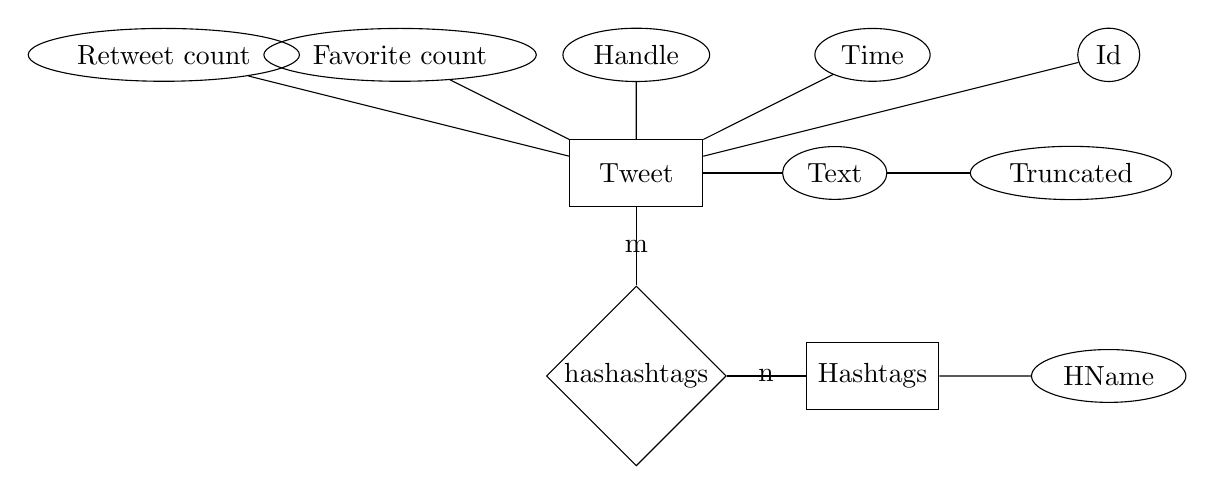
\begin{tikzpicture}
  \node[entity] (node1) {Tweet}
    [grow=up,sibling distance=3cm]
    child {node[attribute] {Id}}
    child {node[attribute] {Time}}
    %child {node[attribute] {text}}
    child {node[attribute] {Handle}}
    child {node[attribute] {Favorite count}}
    child {node[attribute] {Retweet count}};
	\node[attribute] (text) [right=of node1] {Text} edge (text)
    	child[grow=right, level distance=3cm] {node[attribute] {Truncated}};
    %child[grow=left,level distance=3cm] {node[attribute] {Attribute 3}};
  % Now place a relation (ID=rel1)
  \node[relationship] (rel1) [below=of node1] {hashashtags};
  % Now the 2nd entity (ID=rel2)
  \node[entity] (node2) [right = of rel1]	{Hashtags}
    [grow=right,level distance=3cm]
  	child {node[attribute] {HName}};
  % Draw an edges
  \path (rel1) edge node {m} (node1)
    edge	 node {n}	(node2);
  \path (node1) edge node {} (node1) edge node {} (text);
\end{tikzpicture}
\caption{M1} \label{fig:M1} Das ER Modell
\end{figure}

\section{Relationales Modell}
Das Relationale Modell beinhaltet die beiden Entitäten Tweets und Hashtags mit ihren Attributen. Zu den Attributen der Tweets aus dem ER-Modell haben wir das Attribut "id" hinzu genommen, um einen eindeutigen Key für die Hashtags zu bekommen. "id" ist ein Zähler, der jedem Tweet der Tabelle eine Nummer zuweist. 
Somit ist der Key für die Tweets "id", für die Relation contains ist der Key auch "id". 
Der Key der Hashtags ist ihr einziges Attribut, ihr Name "HName". 

Relationales Modell:
\begin{itemize}
\item Tweets(\ handle, text, trancated, time, retweet\_count, favorite\_count,id) 
\item Contains(\ HName, id)
\item Hashtags(\ HName)
\end{itemize}

\section{Datenbank erstellen}
\begin{verbatim}
~$ sudo -u postgres createdb election
~$ sudo -u postgres psql -l
                                  List of databases
   Name    |  Owner   | Encoding |   Collate   |    Ctype    |   Access privileges   
-----------+----------+----------+-------------+-------------+-----------------------
 election  | postgres | UTF8     | de_DE.UTF-8 | de_DE.UTF-8 | 
 postgres  | postgres | UTF8     | de_DE.UTF-8 | de_DE.UTF-8 | 
 template0 | postgres | UTF8     | de_DE.UTF-8 | de_DE.UTF-8 | =c/postgres          +
           |          |          |             |             | postgres=CTc/postgres
 template1 | postgres | UTF8     | de_DE.UTF-8 | de_DE.UTF-8 | =c/postgres          +
           |          |          |             |             | postgres=CTc/postgres
(4 rows)

$ 
\end{verbatim}

%\bibliographystyle{alpha}
%\bibliography{sample}
\end{document}
